\documentclass[tikz,border=5mm]{standalone}
\usepackage{tikz}
\usepackage{amsmath} % Added for the \text command
\usetikzlibrary{arrows.meta, positioning, calc} % Load calc library for coordinate calculations

\begin{document}

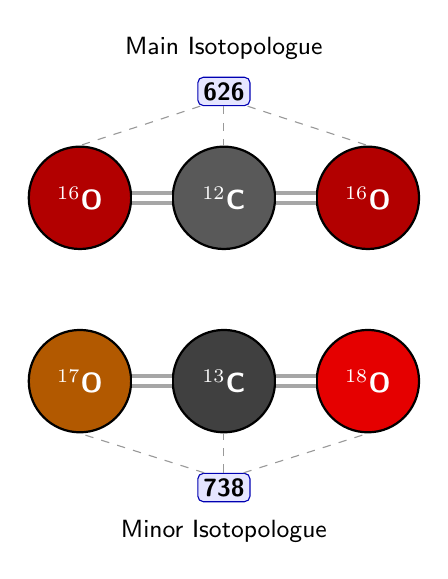
\begin{tikzpicture}
   [
      % Style for the atom: circle, thick border, min size, and font settings
      % The 'fill' is now applied separately, not as part of the style's arguments
      atom/.style={circle, draw, thick, minimum size=1.3cm, font=\sffamily\bfseries\color{white}},
      % Style for the double bond
      bond/.style={double, double distance=2pt, line width=1.5pt, gray!70},
      % Style for the main text labels
      label node/.style={text=black, font=\sffamily\small},
      % Style for the guide lines
      guide line/.style={thin, gray!80, dashed},
      % Style for the blue number boxes
      number box/.style={rectangle, draw=blue!70!black, fill=blue!10, rounded corners=2pt, inner sep=2pt, font=\sffamily\bfseries\small}
   ]

    % =======================================================
    % Top Molecule: Main Isotopologue (12C, 16O, 16O) - 626
    % =======================================================

    % Position the atoms. The labels are now inside the nodes.
    % We apply the 'atom' style and the 'fill' color separately.
    % We use \text{} inside math mode for the element symbols.
    \node[atom, fill=red!70!black] (O1_top) {$^{16}\text{O}$};
    \node[atom, fill=gray!70!black, right=0.5cm of O1_top] (C_top) {$^{12}\text{C}$};
    \node[atom, fill=red!70!black, right=0.5cm of C_top] (O2_top) {$^{16}\text{O}$};

    % Bonds
    \draw[bond] (O1_top) -- (C_top);
    \draw[bond] (C_top) -- (O2_top);

    % Isotopologue Designation (626) - Placed slightly closer to the molecule
    \node[number box, above=0.5cm of C_top.north] (num626) {626};
    
    % Guide lines from the number box to each atom
    % We use the calc library ($(...) + (...)_ to offset the start/end points
    \draw[guide line] ($(num626.south) - (0.3cm, 0)$) -- (O1_top.north);
    \draw[guide line] (num626.south) -- (C_top.north);
    \draw[guide line] ($(num626.south) + (0.3cm, 0)$) -- (O2_top.north);

    % =======================================================
    % Bottom Molecule: Minor Isotopologue (13C, 17O, 18O) - 738
    % =======================================================

    % Position the atoms (below the top one)
    \node[atom, fill=orange!70!black, below=1cm of O1_top] (O1_bottom) {$^{17}\text{O}$};
    \node[atom, fill=gray!50!black, right=0.5cm of O1_bottom] (C_bottom) {$^{13}\text{C}$};
    \node[atom, fill=red!90!black, right=0.5cm of C_bottom] (O2_bottom) {$^{18}\text{O}$};

    % Bonds
    \draw[bond] (O1_bottom) -- (C_bottom);
    \draw[bond] (C_bottom) -- (O2_bottom);

    % Isotopologue Designation (738) - Placed slightly closer
    \node[number box, below=0.5cm of C_bottom.south] (num738) {738};
    
    % Guide lines from the number box to each atom
    \draw[guide line] ($(num738.north) - (0.25cm, 0)$) -- (O1_bottom.south);
    \draw[guide line] (num738.north) -- (C_bottom.south);
    \draw[guide line] ($(num738.north) + (0.25cm, 0)$) -- (O2_bottom.south);

    % Labels for Main/Minor Isotopologue - Placed slightly closer
    \node[label node, above=0.1cm of num626.north] {Main Isotopologue};
    \node[label node, below=0.1cm of num738.south] {Minor Isotopologue};

\end{tikzpicture}


\end{document}